\documentclass{article}
\usepackage[left=40mm, right=40mm, top=30mm, bottom=30mm]{geometry}
\usepackage[utf8]{inputenc}
\usepackage[italian]{babel}
\usepackage{amssymb}
\usepackage{amsthm}
\usepackage{graphics}
\usepackage{amsfonts}
\usepackage{listings}
\usepackage{amsmath}
\usepackage{amstext}
\usepackage{engrec}
\usepackage{rotating}
\usepackage{verbatim}
\usepackage[safe,extra]{tipa}
\usepackage{multirow}
\usepackage{hyperref}
\usepackage{microtype}
\usepackage{enumerate}
\usepackage{physics}
\usepackage{braket}
\usepackage{multicol}
%\usepackage{mhchem}
\usepackage{marginnote}
%\usepackage{pgfplots}
\usepackage{cancel}
\usepackage{polynom}
\usepackage{booktabs}
\usepackage{enumitem}
\usepackage{framed}
\usepackage{pdfpages}
\usepackage{algorithm}
% \usepackage{algpseudocode}
\usepackage[cache=false]{minted}
\usepackage{mathtools}
\usepackage[noend]{algpseudocode}
\title{Hands-On}
\author{Davide Cozzi, Fabio Pirovano, Viola Rillosi}
\date{04/05/2022}
\begin{document}

\maketitle
\section*{Formule}
\[a_\mu(X(t))=c_\mu h_\mu(t),\,\,
  a_0(X)=\sum_{\mu=1}^Ma_\mu(X),\,\,
  \tau=\frac{1}{a_0(X)}\ln\frac{1}{r_1}\]
\begin{table}[H]
    \centering
    \begin{tabular}{c|c}
      Reagenti & $h_\mu$\\
      \hline
      \hline
      $S_j$ & $h_\mu=X_j$\\
      $S_j+S_k, \,\,j\neq k$ & $h_\mu=X_jX_k$\\
      $2S_j$ & $h_\mu=\frac{X_j(X_j-1)}{2}$
    \end{tabular}
  \end{table}
\section*{Esercizio}
Sia dato il seguente sistema con 3 specie e 4 reazioni:
\[\mathcal{S}=\{S_1,S_2,S_3\}\]
\begin{table}[H]
  \centering
  \begin{tabular}{c|c|c|c}
    \# & \textbf{Reagenti} & \textbf{Prodotti} & \textbf{Costanti}\\
    \hline
    \hline
    $R_1$ & $S_1+S_1$ & $S_2$ & $c_1=1.0$\\
    $R_2$ & $S_2$ & $S_1+S_1$ & $c_2=0.1$\\
    $R_3$ & $S_2+S_2$ & $S_3$ & $c_3=0.5$\\
    $R_4$ & $S_1+S_3$ & $S_2$ & $c_4=10.0$\\
  \end{tabular}
\end{table}
Con quindi i seguenti \textit{state-change vector}:
\begin{multicols}{2}
  \begin{itemize}
    \item $v_1=(-2,+1,0)$
    \item $v_2=(+1,-1,0)$
    \item $v_3=(0,-2,+1)$
    \item $v_4=(-1,+1,-1)$
  \end{itemize}
\end{multicols}
\newpage
Si ha la simulazione di 5 step di simulazione tramite \textit{SSA} partendo
dallo stato iniziale:
\[X(0)=(10,0,0)\]
\begin{enumerate}[label=\roman*)]
  \item \textbf{al tempo $\mathbf{t=0}$} si calcolano, avendo $X=X(0)=(10,0,0)$:
  \begin{multicols}{2}
    \begin{itemize}
      \item {\small{$a_1(X)=c_1h_1(t)=1.0\cdot\frac{10(10-1)}{2}=45$}}
      \item $a_2(X)=c_2h_2(t)=0.1\cdot 0=0$
      \item $a_3(X)=c_3h_3(t)=0.5\cdot \frac{0(0-1)}{2}=0$
      \item $a_4(X)=c_4h_4(t)=10.0\cdot 10 \cdot 0=0$
    \end{itemize}
  \end{multicols}
  Si ha quindi:
  \[a_0(X)=45+0+0+0=45\]
  Si procede quindi generando i due numeri pseudocasuali:
  \begin{multicols}{2}
    \begin{itemize}
      \item $r_1=0.35$
      \item $r_2=0.84$
    \end{itemize}
  \end{multicols}
  Si calcola $\tau$:
  \[\tau=\frac{1}{45}\ln\frac{1}{0.35}=0.02\]
  Avendo quindi che il tempo $t$ viene aggiornato come:
  \[t=0+0.02=0.02\]
  Si calcolano i vari $\frac{a_\mu(X)}{a_0(X)}$:
  \begin{multicols}{2}
    \begin{itemize}
      \item $\frac{a_1(X)}{a_0(X)}=\frac{45}{45}=1$
      \item $\frac{a_2(X)}{a_0(X)}=\frac{0}{45}=0$
      \item $\frac{a_3(X)}{a_0(X)}=\frac{0}{45}=0$
      \item $\frac{a_4(X)}{a_0(X)}=\frac{0}{45}=0$
    \end{itemize}
  \end{multicols}
  Avendo quindi:
  \begin{figure}[H]
    \centering
    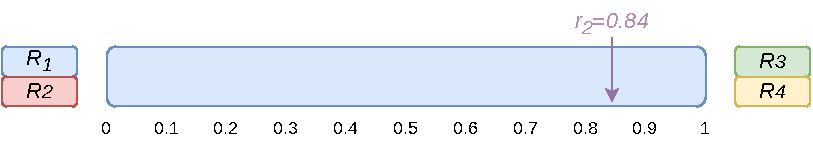
\includegraphics[scale = 0.8]{img/t1.pdf}
  \end{figure}
  E quindi si avrà, avendo $r_2=0.84$:
  \[\mu=1\]
  E quindi si aggiorna lo stato $X$:
  \[X(0) = (10,0,0) \Rightarrow X(0.02) = (10-2,0+1,0) = (8,1,0)\]
  \newpage
  \item \textbf{al tempo $\mathbf{t=0.02}$} si calcolano, avendo
  $X=X(0.02)=(8,1,0)$: 
  \begin{multicols}{2}
    \begin{itemize}
      \item $a_1(X)=c_1h_1(t)=1.0\cdot\frac{8(8-1)}{2}=28$
      \item $a_2(X)=c_2h_2(t)=0.1\cdot 1=0.1$
      \item $a_3(X)=c_3h_3(t)=0.5\cdot \frac{1(1-1)}{2}=0$
      \item $a_4(X)=c_4h_4(t)=10.0\cdot 10 \cdot 0=0$
    \end{itemize}
  \end{multicols}
  Si ha quindi:
  \[a_0(X)=28+0.1+0+0=28.1\]
  Si procede quindi generando i due numeri pseudocasuali:
  \begin{multicols}{2}
    \begin{itemize}
      \item $r_1=0.04$
      \item $r_2=0.20$
    \end{itemize}
  \end{multicols}
  Si calcola $\tau$:
  \[\tau=\frac{1}{28.1}\ln\frac{1}{0.04}=0.11\]
  Avendo quindi che il tempo $t$ viene aggiornato come:
  \[t=0.02+0.11=0.13\]
  Si calcolano i vari $\frac{a_\mu(X)}{a_0(X)}$:
  \begin{multicols}{2}
    \begin{itemize}
      \item $\frac{a_1(X)}{a_0(X)}=\frac{28}{28.1}=0.996$
      \item $\frac{a_2(X)}{a_0(X)}=\frac{0.1}{28.1}=0.004$
      \item $\frac{a_3(X)}{a_0(X)}=\frac{0}{28.1}=0$
      \item $\frac{a_4(X)}{a_0(X)}=\frac{0}{28.1}=0$
    \end{itemize}
  \end{multicols}
  Avendo quindi:
  \begin{figure}[H]
    \centering
    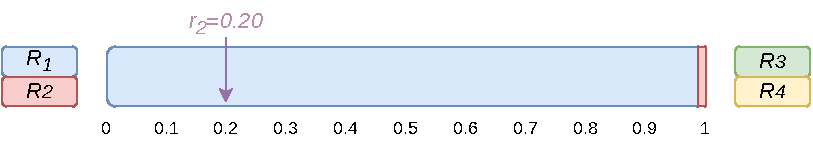
\includegraphics[scale = 0.8]{img/t2.pdf}
  \end{figure}
  E quindi si avrà, avendo $r_2=0.20$:
  \[\mu=1\]
  E quindi si aggiorna lo stato $X$:
  \[X(0.02) = (8,1,0) \Rightarrow X(0.13) = (8-2,1+1,0) = (6,2,0)\]
  \newpage
  \item \textbf{al tempo $\mathbf{t=0.13}$} si calcolano, avendo
  $X=X(0.13)=(6,2,0)$: 
  \begin{multicols}{2}
    \begin{itemize}
      \item $a_1(X)=c_1h_1(t)=1.0\cdot\frac{6(6-1)}{2}=15$
      \item $a_2(X)=c_2h_2(t)=0.1\cdot 2=0.2$
      \item $a_3(X)=c_3h_3(t)=0.5\cdot \frac{2(2-1)}{2}=0.5$
      \item $a_4(X)=c_4h_4(t)=10.0\cdot 10 \cdot 0=0$
    \end{itemize}
  \end{multicols}
  Si ha quindi:
  \[a_0(X)=15+0.2+0.5+0=15.7\]
  Si procede quindi generando i due numeri pseudocasuali:
  \begin{multicols}{2}
    \begin{itemize}
      \item $r_1=0.73$
      \item $r_2=0.85$
    \end{itemize}
  \end{multicols}
  Si calcola $\tau$:
  \[\tau=\frac{1}{15.7}\ln\frac{1}{0.73}=0.02\]
  Avendo quindi che il tempo $t$ viene aggiornato come:
  \[t=0.13+0.02=0.15\]
  Si calcolano i vari $\frac{a_\mu(X)}{a_0(X)}$:
  \begin{multicols}{2}
    \begin{itemize}
      \item $\frac{a_1(X)}{a_0(X)}=\frac{15}{15.7}=0.96$
      \item $\frac{a_2(X)}{a_0(X)}=\frac{0.2}{15.7}=0.01$
      \item $\frac{a_3(X)}{a_0(X)}=\frac{0.5}{15.7}=0.03$
      \item $\frac{a_4(X)}{a_0(X)}=\frac{0}{15.7}=0$
    \end{itemize}
  \end{multicols}
  Avendo quindi:
  \begin{figure}[H]
    \centering
    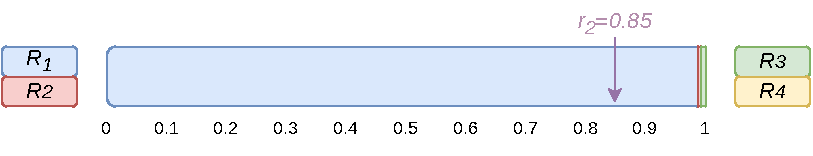
\includegraphics[scale = 0.8]{img/t3.pdf}
  \end{figure}
  E quindi si avrà, avendo $r_2=0.85$:
  \[\mu=1\]
  E quindi si aggiorna lo stato $X$:
  \[X(0.13) = (6,2,0) \Rightarrow X(0.15) = (6-2,2+1,0) = (4,3,0)\]
  \newpage
  \item \textbf{al tempo $\mathbf{t=0.15}$} si calcolano, avendo
  $X=X(0.13)=(4,3,0)$: 
  \begin{multicols}{2}
    \begin{itemize}
      \item $a_1(X)=c_1h_1(t)=1.0\cdot\frac{4(4-1)}{2}=6$
      \item $a_2(X)=c_2h_2(t)=0.1\cdot 3=0.3$
      \item $a_3(X)=c_3h_3(t)=0.5\cdot \frac{3(3-1)}{2}=1.5$
      \item $a_4(X)=c_4h_4(t)=10.0\cdot 10 \cdot 0=0$
    \end{itemize}
  \end{multicols}
  Si ha quindi:
  \[a_0(X)=6+0.3+1.5+0=7.8\]
  Si procede quindi generando i due numeri pseudocasuali:
  \begin{multicols}{2}
    \begin{itemize}
      \item $r_1=0.11$
      \item $r_2=0.44$
    \end{itemize}
  \end{multicols}
  Si calcola $\tau$:
  \[\tau=\frac{1}{7.8}\ln\frac{1}{0.11}=0.28\]
  Avendo quindi che il tempo $t$ viene aggiornato come:
  \[t=0.15+0.28=0.43\]
  Si calcolano i vari $\frac{a_\mu(X)}{a_0(X)}$:
  \begin{multicols}{2}
    \begin{itemize}
      \item $\frac{a_1(X)}{a_0(X)}=\frac{6}{7.8}=0.77$
      \item $\frac{a_2(X)}{a_0(X)}=\frac{0.3}{7.8}=0.04$
      \item $\frac{a_3(X)}{a_0(X)}=\frac{1.5}{7.8}=0.19$
      \item $\frac{a_4(X)}{a_0(X)}=\frac{0}{7.8}=0$
    \end{itemize}
  \end{multicols}
  Avendo quindi:
  \begin{figure}[H]
    \centering
    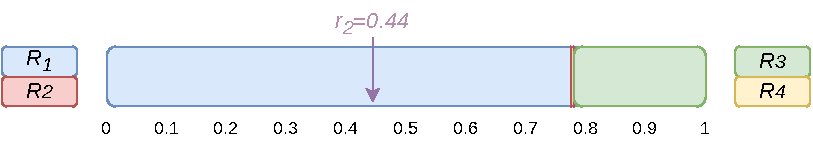
\includegraphics[scale = 0.8]{img/t4.pdf}
  \end{figure}
  E quindi si avrà, avendo $r_2=0.44$:
  \[\mu=1\]
  E quindi si aggiorna lo stato $X$:
  \[X(0.15) = (4,3,0) \Rightarrow X(0.43) = (4-2,3+1,0) = (2,4,0)\]
  \newpage
  \item \textbf{al tempo $\mathbf{t=0.43}$} si calcolano, avendo
  $X=X(0.13)=(2,4,0)$: 
  \begin{multicols}{2}
    \begin{itemize}
      \item $a_1(X)=c_1h_1(t)=1.0\cdot\frac{2(2-1)}{2}=1$
      \item $a_2(X)=c_2h_2(t)=0.1\cdot 4=0.4$
      \item $a_3(X)=c_3h_3(t)=0.5\cdot \frac{4(4-1)}{2}=3$
      \item $a_4(X)=c_4h_4(t)=10.0\cdot 10 \cdot 0=0$
    \end{itemize}
  \end{multicols}
  Si ha quindi:
  \[a_0(X)=1+0.4+3+0=4.4\]
  Si procede quindi generando i due numeri pseudocasuali:
  \begin{multicols}{2}
    \begin{itemize}
      \item $r_1=0.56$
      \item $r_2=0.30$
    \end{itemize}
  \end{multicols}
  Si calcola $\tau$:
  \[\tau=\frac{1}{4.4}\ln\frac{1}{0.56}=0.13\]
  Avendo quindi che il tempo $t$ viene aggiornato come:
  \[t=0.43+0.13=0.56\]
  Si calcolano i vari $\frac{a_\mu(X)}{a_0(X)}$:
  \begin{multicols}{2}
    \begin{itemize}
      \item $\frac{a_1(X)}{a_0(X)}=\frac{1}{4.4}=0.23$
      \item $\frac{a_2(X)}{a_0(X)}=\frac{0.4}{4.4}=0.09$
      \item $\frac{a_3(X)}{a_0(X)}=\frac{3}{4.4}=0.68$
      \item $\frac{a_4(X)}{a_0(X)}=\frac{0}{4.4}=0$
    \end{itemize}
  \end{multicols}
  Avendo quindi:
  \begin{figure}[H]
    \centering
    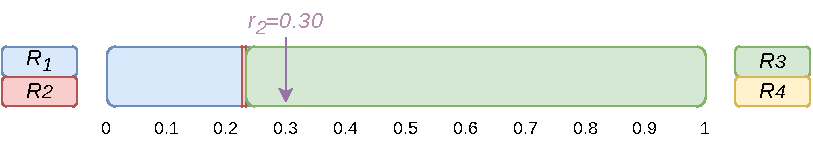
\includegraphics[scale = 0.8]{img/t5.pdf}
  \end{figure}
  E quindi si avrà, avendo $r_2=0.30$:
  \[\mu=3\]
  E quindi si aggiorna lo stato $X$:
  \[X(0.43) = (2,4,0) \Rightarrow X(0.46) = (2,4-2,0+1) = (2,2,1)\]
\end{enumerate}
\end{document}
